\section{Simplified architecture}
\textit{Figure \ref{fig:simplified_architecture}} shows a complete view of the entities composing the simplified architecture for the Interconnected project (that can be compared to the full architecture shown in \textit{figure \ref{fig:architecture_complete}}).

\begin{figure}[!ht]
    \centering
    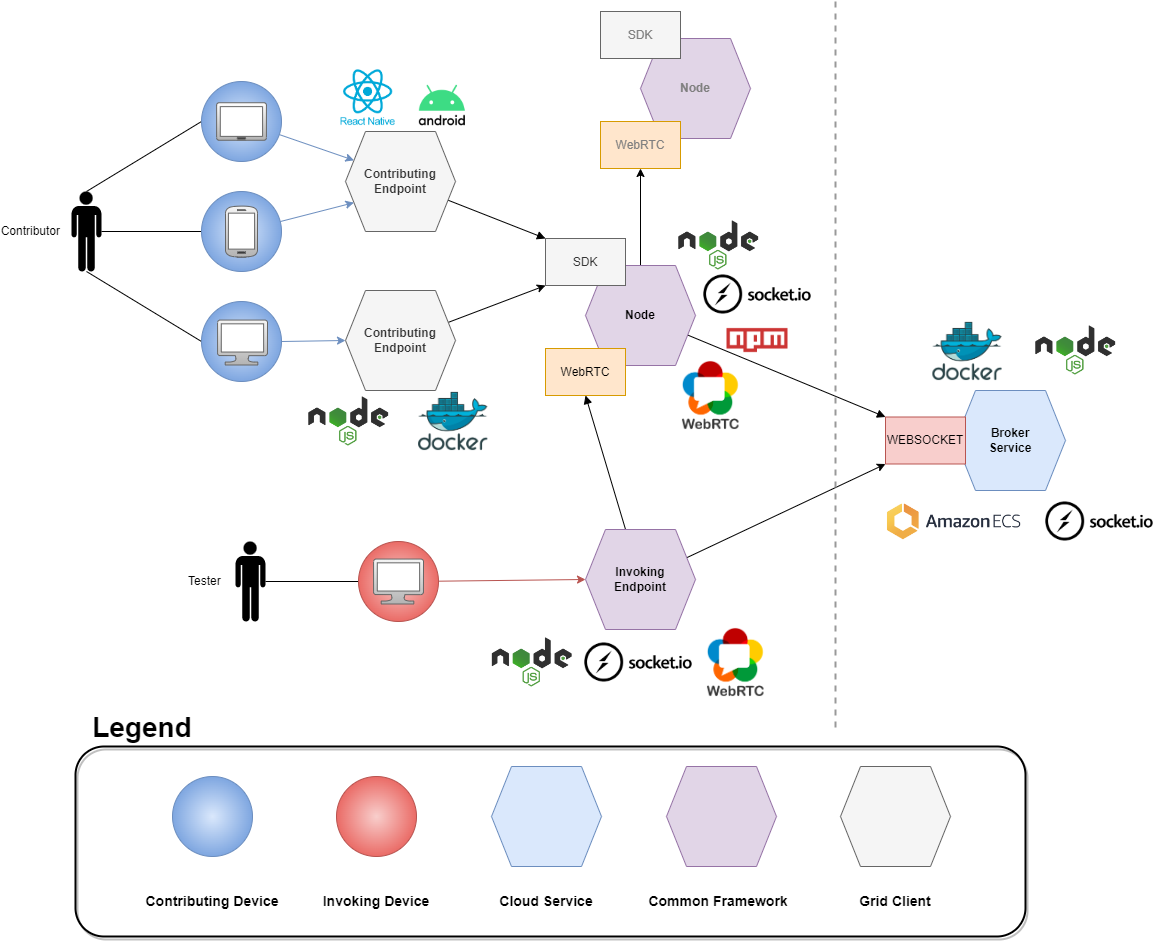
\includegraphics[width=\linewidth]{document/chapters/chapter_7/images/simplified_architecture.png}
    \caption{Complete view of the simplified prototype's architecture}
    \label{fig:simplified_architecture}
\end{figure}

\vspace{10mm}

All the entities composing the architecture are implemented using technologies based on Node.js which offers useful, popular and well maintained frameworks as well as an easy to use concurrency model based on an event loop.

\subsection{Broker Service}
The only Cloud Service present in this simplified architecture is the Broker Service; since only one instance (with a static address) of such Cloud Service is required to sustain the workload of the few devices connected, a dynamic handling and discovery of multiple instances is thus not required. As a direct consequence of that, the complementary entities that handled the dynamic system for scalability (Grid Master Service, Broker Discovery Service and Grid Services Gateway Service) are not needed and thus Nodes and Invoking Endpoints communicate directly with the Broker Service without first undergoing the discovery processes described in \textit{section \ref{use_cases_satisfaction}}.

The prototype's Broker Service is implemented by using the Typescript language and utilizes Socket.io in order to create a web server that is reachable via WebSocket protocol; through the use of this technology, Invoking Endpoints are able to deposit requests for the recruitment of Nodes that will be used to perform computations. The messages involved in the recruiting process and the general Grid connection will be discussed in \textit{section \ref{coordination}}.

In order to have a running instance of the Broker Service that also has a static address reachable from anywhere, a Docker image is created which, in turn, is executed in a container through the use of Amazon ECS (Elastic Container Service). More details about the deployment of this entity will be discussed later in \textit{section \ref{devops}}.

\subsection{Interconnected Node}\label{interconnected_node}
The Node entity, which in the Interconnected project takes the name of "Interconnected Node", contains all the logic regarding the contribution of a device, and it is distributed through NPM as a Node.js dependency that is then integrated in the concrete clients targeting various devices.

Interconnected Node is also developed by using the Typescript language and, being this a client in the WebSocket connection to the Broker Service, it utilizes the client-side implementation of the Socket.io framework.

The P2P connectivity requirements are concretized through the use of the WebRTC (Real-Time Communication for the Web) protocol; such communication standard it is used to send audio and video data among peers, as well as any kind of structured non-media data. In order for the peers to establish the connection, first the signaling process needs to be completed: the peers, through a third intermediary (the Broker Service), exchange some information required for the connection to happen; the Peer that initializes the connection creates an SDP (Signaling Description Protocol) object, denominated "offer". When the other Peer receives such data, it also creates its SDP object denominated "answer". Once each Peers posses both generated SDP data, they finalize the connection exchanging some ICE (Interactive Connectivity Establishment) candidates; such ICE candidates needs to be specified when realizing a WebRTC connection since they are the actual servers that allow the P2P connection. There are two types of servers involved:
\begin{itemize}
    \item \textbf{STUN} (Session Traversal Utilities for NAT)\\
    Used by Peers that resides behind the same NAT; through this server the IP info of each Peer are retrieved and a direct P2P connection can be established.
    \item \textbf{TURN} (Traversal Using Relays around NAT)\\
    Used by Peers that resides in different NATs; through this server the limitations of a NAT are overcome, creating an indirect P2P connection that uses the TURN server to forward the messages among the two Peers.
\end{itemize}

\begin{figure}[!ht]
    \centering
    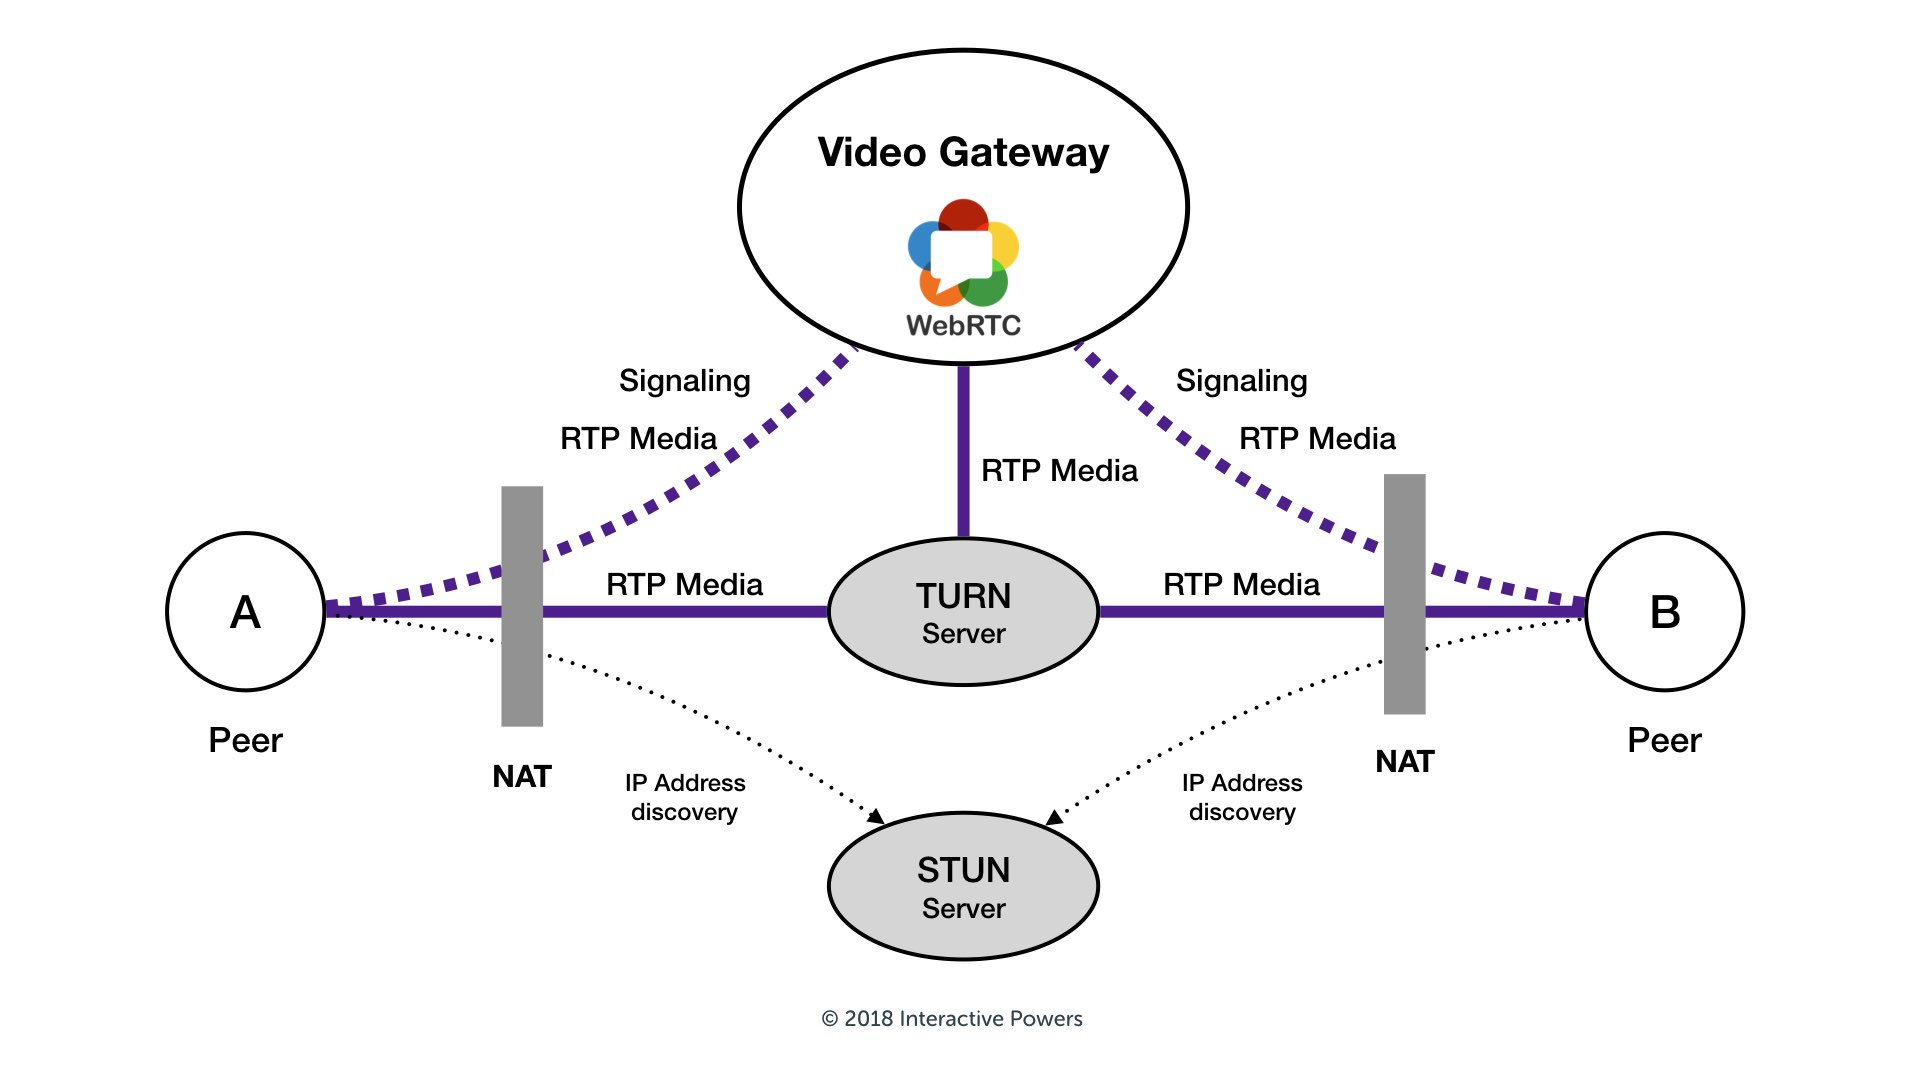
\includegraphics[scale=0.15]{document/chapters/chapter_7/images/webrtc.jpeg}
    \caption{WebRTC - STUN and TURN servers \cite{stun_and_turn_servers}}
    \label{fig:webrtc}
\end{figure}

Free STUN and TURN servers (used by this prototype) are available to the general public thanks to the \textbf{\href{https://www.metered.ca/tools/openrelay/}{Open Relay}} initiative.

There are both a \textbf{\href{https://www.npmjs.com/package/wrtc}{Desktop implementation}} and a \textbf{\href{https://www.npmjs.com/package/react-native-webrtc}{React Native implementation}} of Node.js modules that allow to perform P2P connections utilizing the WebRTC protocol but, despite functioning in the same way and exposing the same interfaces with identical methods, the Desktop implementation does not work on React Native and vice versa. In order to circumvent this problem, the object handling the P2P connection is wrapped in an interface that needs to be concretized in the specific Desktop and Mobile implementations (\textit{figure \ref{fig:p2p_wrapper}}); this also allow to add some domain-specific logic, assigning to the Peer that initializes the connection the "Master" role and the "Slave" role to the other Peer. 

\begin{figure}[!ht]
    \centering
    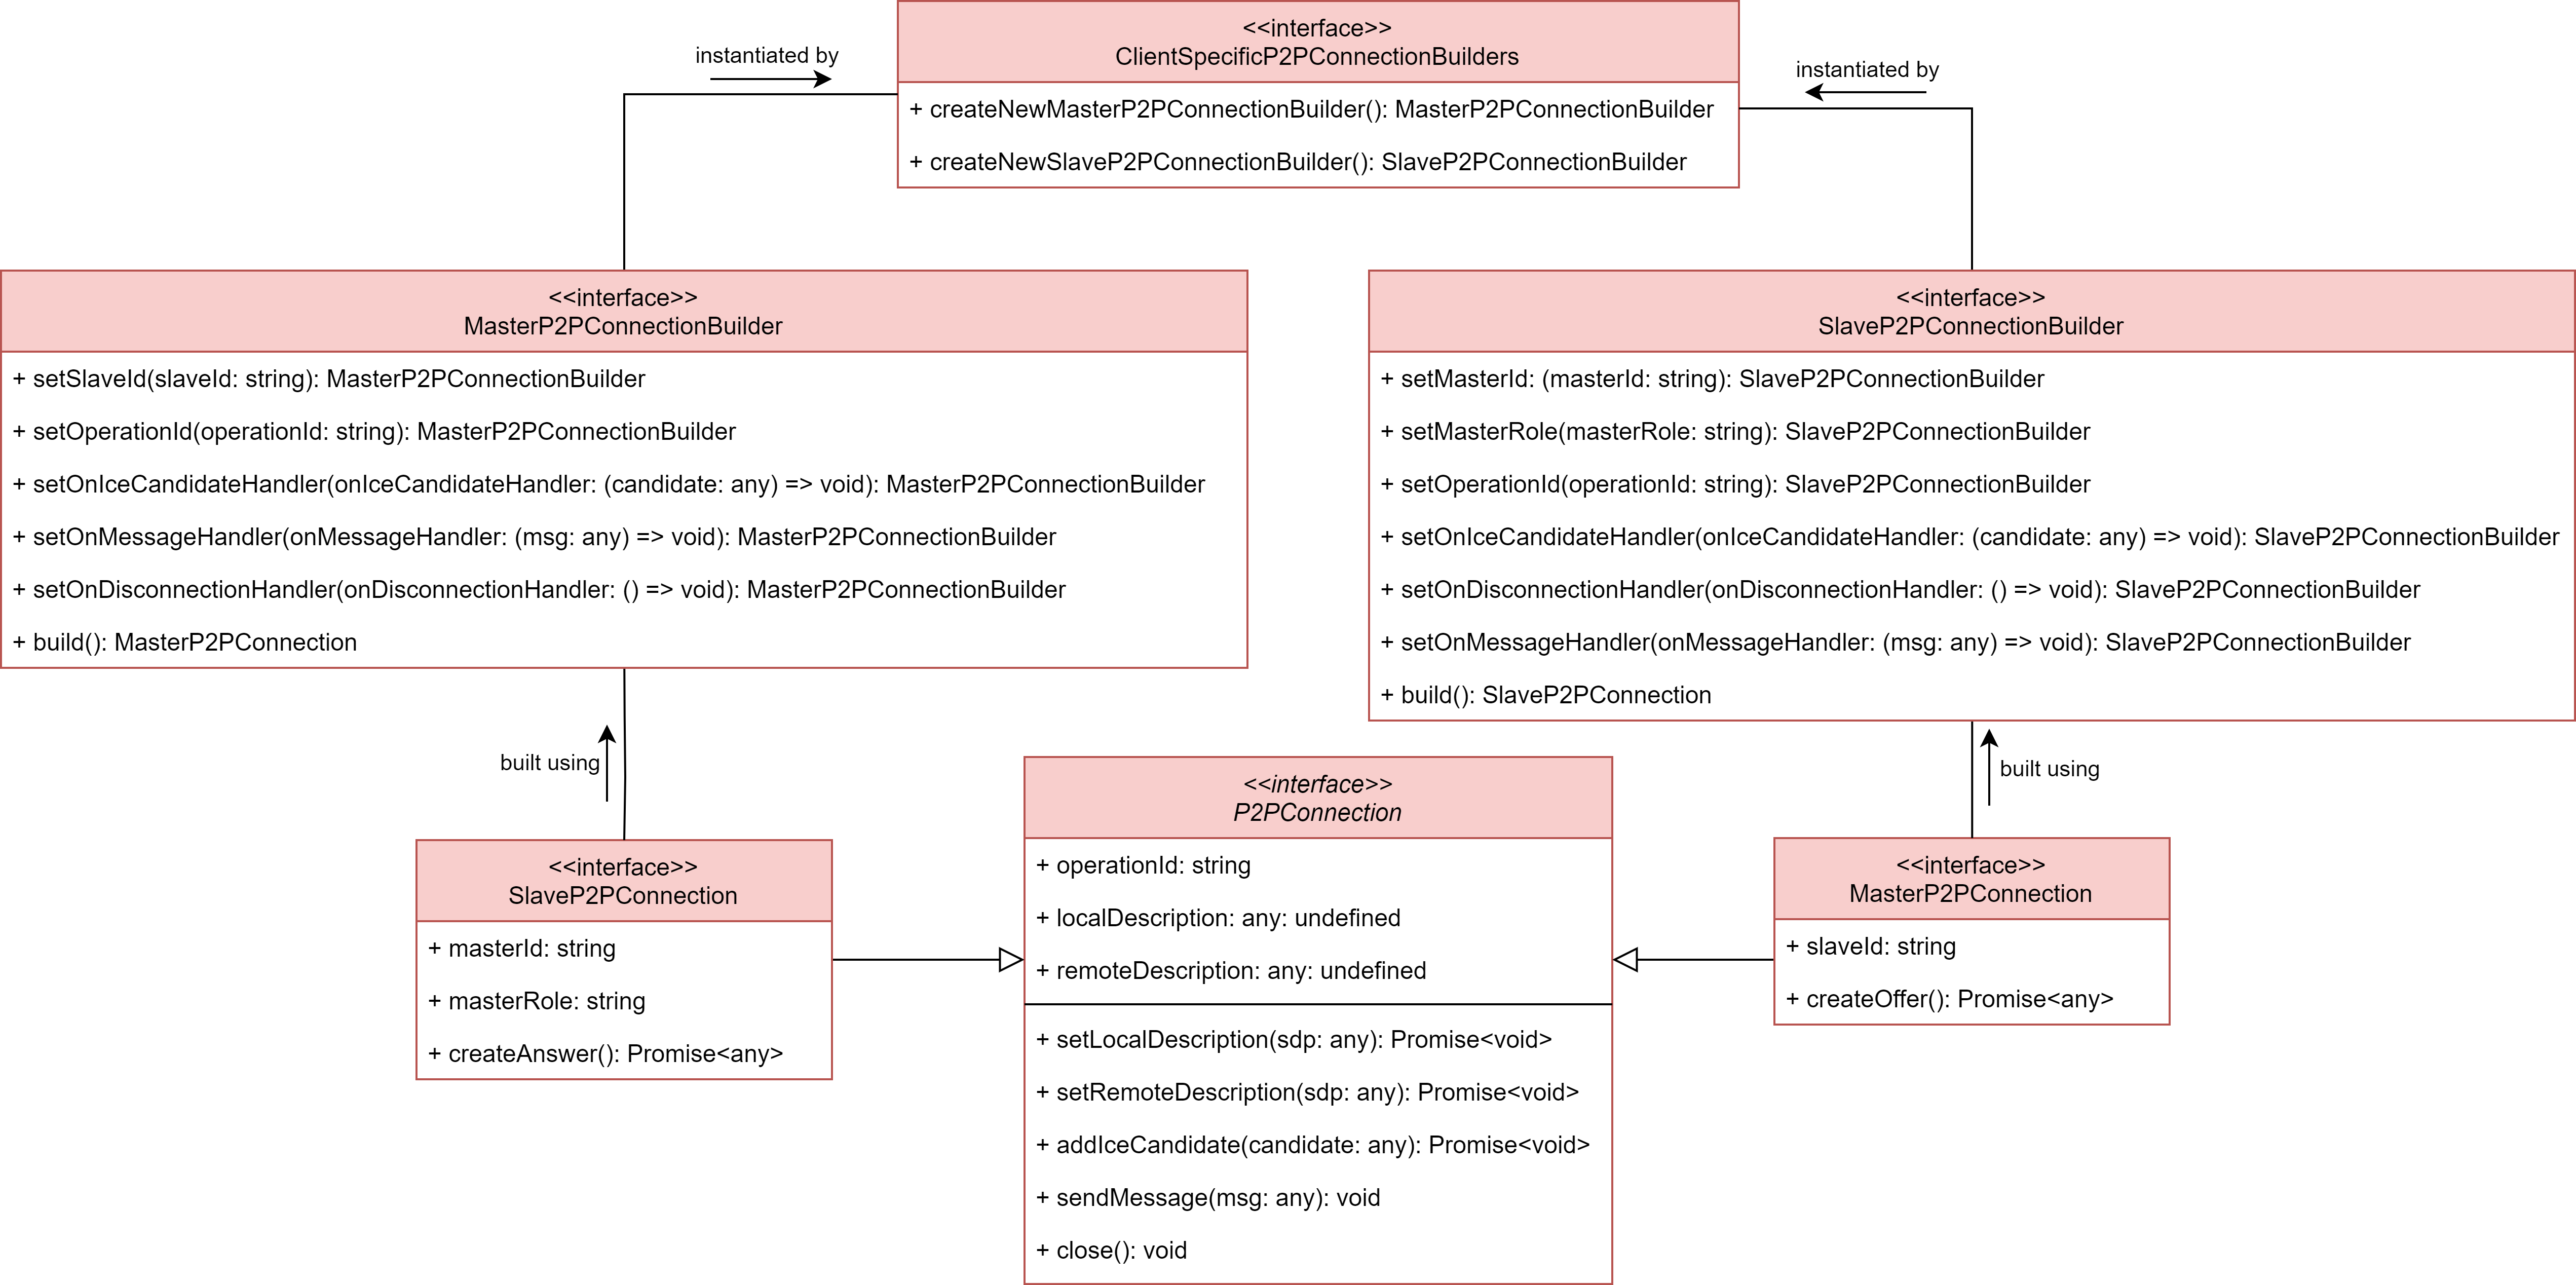
\includegraphics[width=\linewidth]{document/chapters/chapter_7/images/p2p_wrapper.png}
    \caption{WebRTC P2P Wrappers and builders}
    \label{fig:p2p_wrapper}
\end{figure}

The construction of the client-specific objects is standardized through the utilization of the Builder pattern, allowing the internal logic of the Interconnected Node to create instances of such objects without actually possessing the concrete implementation. The P2P Builders (along with an unique device identifier) will then be passed at construction time to the InterconnectedNode Facade (\textit{\ref{fig:interconnected_node_facade}}) which exposes simple methods to interact with the core logic, hiding its complexity and requiring the specific client only to deal with presentational aspects and device-specific responsibilities.

\begin{figure}[!ht]
    \centering
    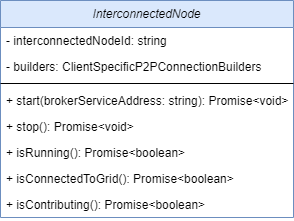
\includegraphics[scale=0.6]{document/chapters/chapter_7/images/interconnected_node_facade.png}
    \caption{Interconnected Node Facade}
    \label{fig:interconnected_node_facade}
\end{figure}

When it comes to the actual computational contribution that the Interconnected Node needs to perform, two key abstractions are present: Job and Task; a Job is an activity that a Slave Peer executes under the guidance of its Master that, after instructing the start of said Job, sends Tasks to execute in that specific Job. This abstraction results in the definition of common interfaces for Job and Task that are then concretized realizing new functionalities that will then be used to execute Grid Services (MapReduceMasterJob, MapReduceMapWorkerJob, etc...); through this mechanism, expanding the support for new Grid Services only requires to define new concrete Jobs and Tasks, realizing their logic and their handlers for the messages exchanged among Nodes.

\subsection{Interconnected Mobile Client}
In this prototype, the mobile incarnation of the Contributing Endpoint takes the name of "Interconnected Mobile Client". The main technology used for realizing this client is React Native (which is also Node.js based); with this framework, it is possible to build mobile applications targeting both Android and iOS devices with just one code base while also taking advantage of most of the modules available on NPM.

Thanks to this Node.js compatibility, the mobile client is able to use the Interconnected Node to connect to the Grid and perform contributions, only requiring to implement previously mentioned client-specific interfaces and to provide an ID for the device (given the limited number of devices in the prototype setting a UUID v4 is generated and used as the ID).

Although React Native also allows targeting iOS devices, this prototype is tested only on Android devices; this limitation is caused by the previously mentioned lack of resources (in particular the unavailability of Apple devices to test it on) but, in theory, the application should also function on iPhones and iPads with little to no changes to the code base.

\begin{figure}[!ht]
    \centering
    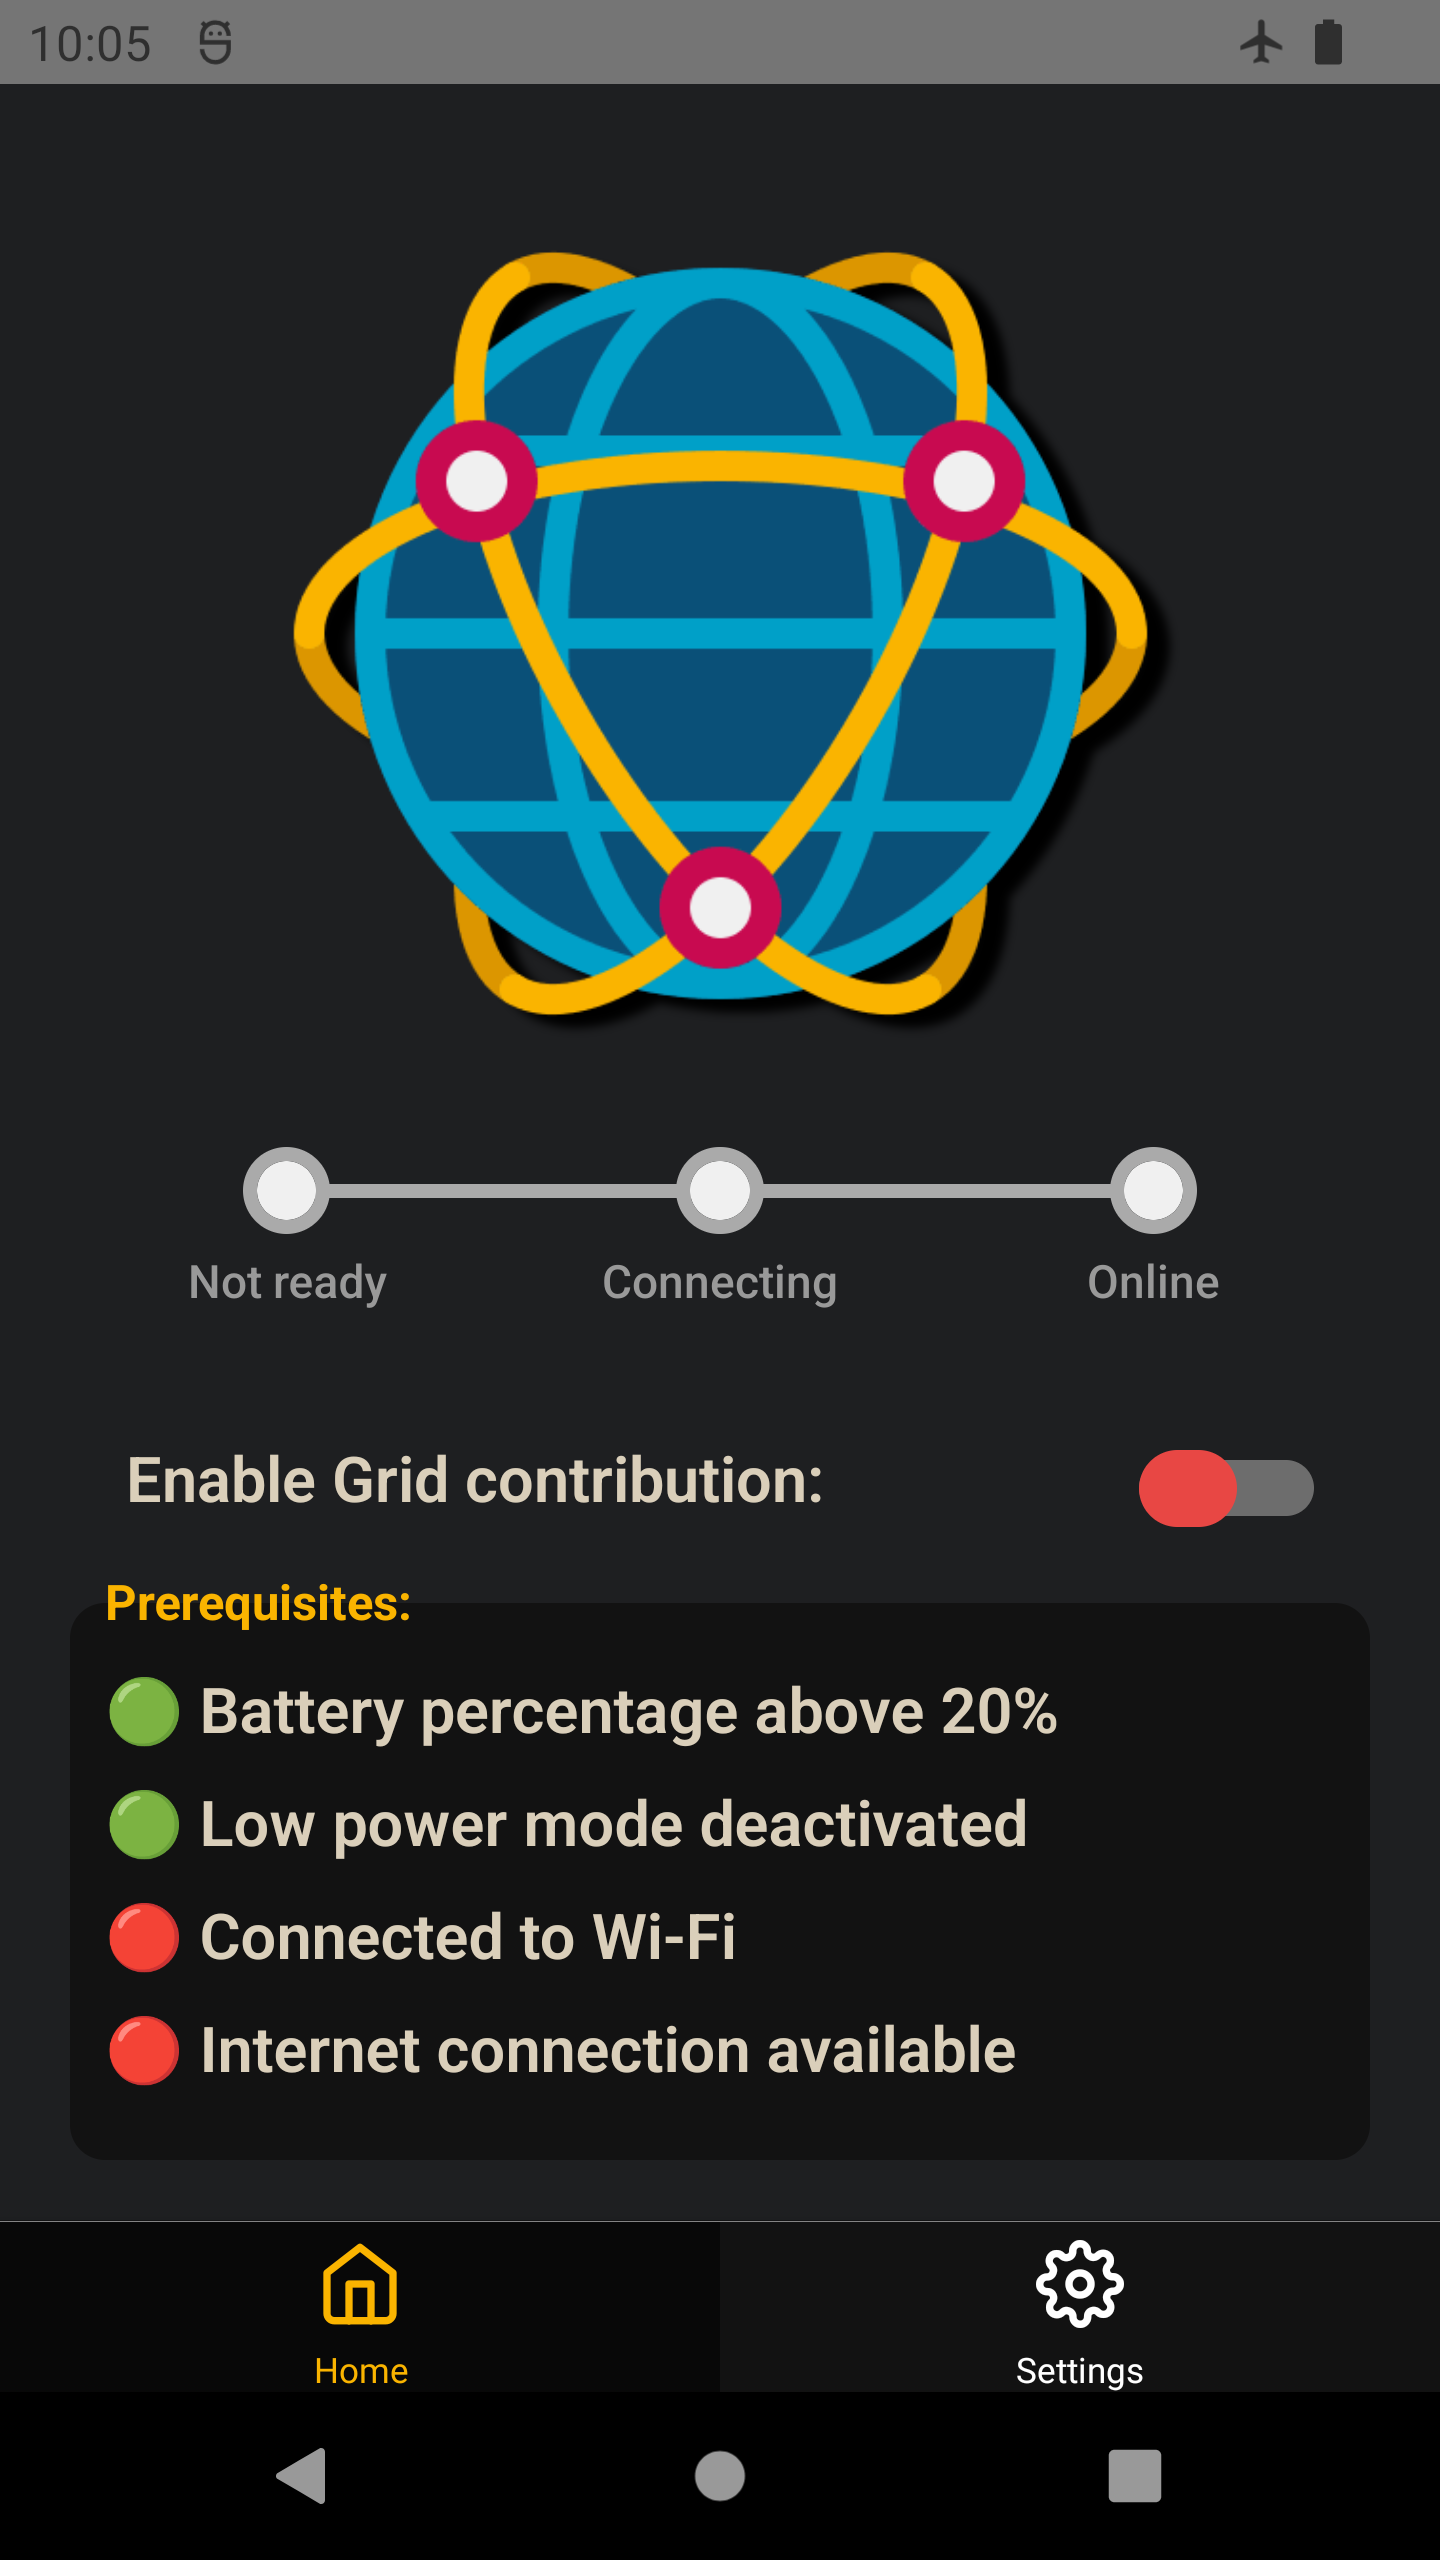
\includegraphics[scale=0.14]{document/chapters/chapter_7/images/interconnected_mobile_home.png}
    \caption{Interconnected Mobile Client}
    \label{fig:interconnected_mobile_home}
\end{figure}

\textit{Figure \ref{fig:interconnected_mobile_home}} shows the GUI of the application: by simply activating the "Enable Grid contribution" switch (\textit{figure \ref{fig:interconnected_mobile_connection}(a)}), the application starts a background process that continues to operate even after the application is closed; Android forces the developer to notify the user of the presence of a background activity by spawning a permanent notification (which can be seen in \textit{figure \ref{fig:notification_contribution}}) that will automatically be removed when the background activity is stopped by disabling the switch.

This background process is responsible for checking a series of conditions (that are listed in the "Prerequisites" section of the GUI) which are necessary for Grid Contribution; when all the conditions are met, the Interconnected Node is started through the use of the previously mentioned Facade exposed by the module. In case even one of the prerequisites is not satisfied anymore, the Interconnected Node is stopped.

\begin{figure}[!ht]
    \centering
    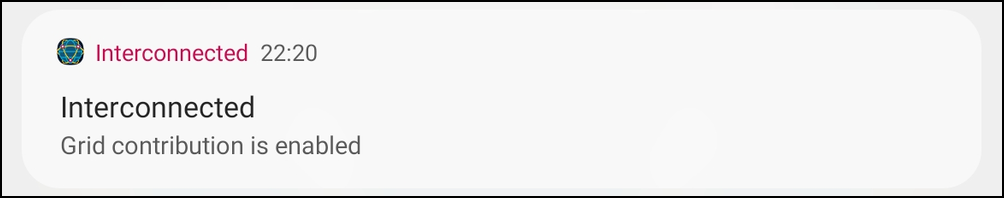
\includegraphics[scale=0.35]{document/chapters/chapter_7/images/notification_contribution.png}
    \caption{Interconnected Mobile Client - Grid contribution enabled notification}
    \label{fig:notification_contribution}
\end{figure}

\begin{figure}[!ht]
    \centering
    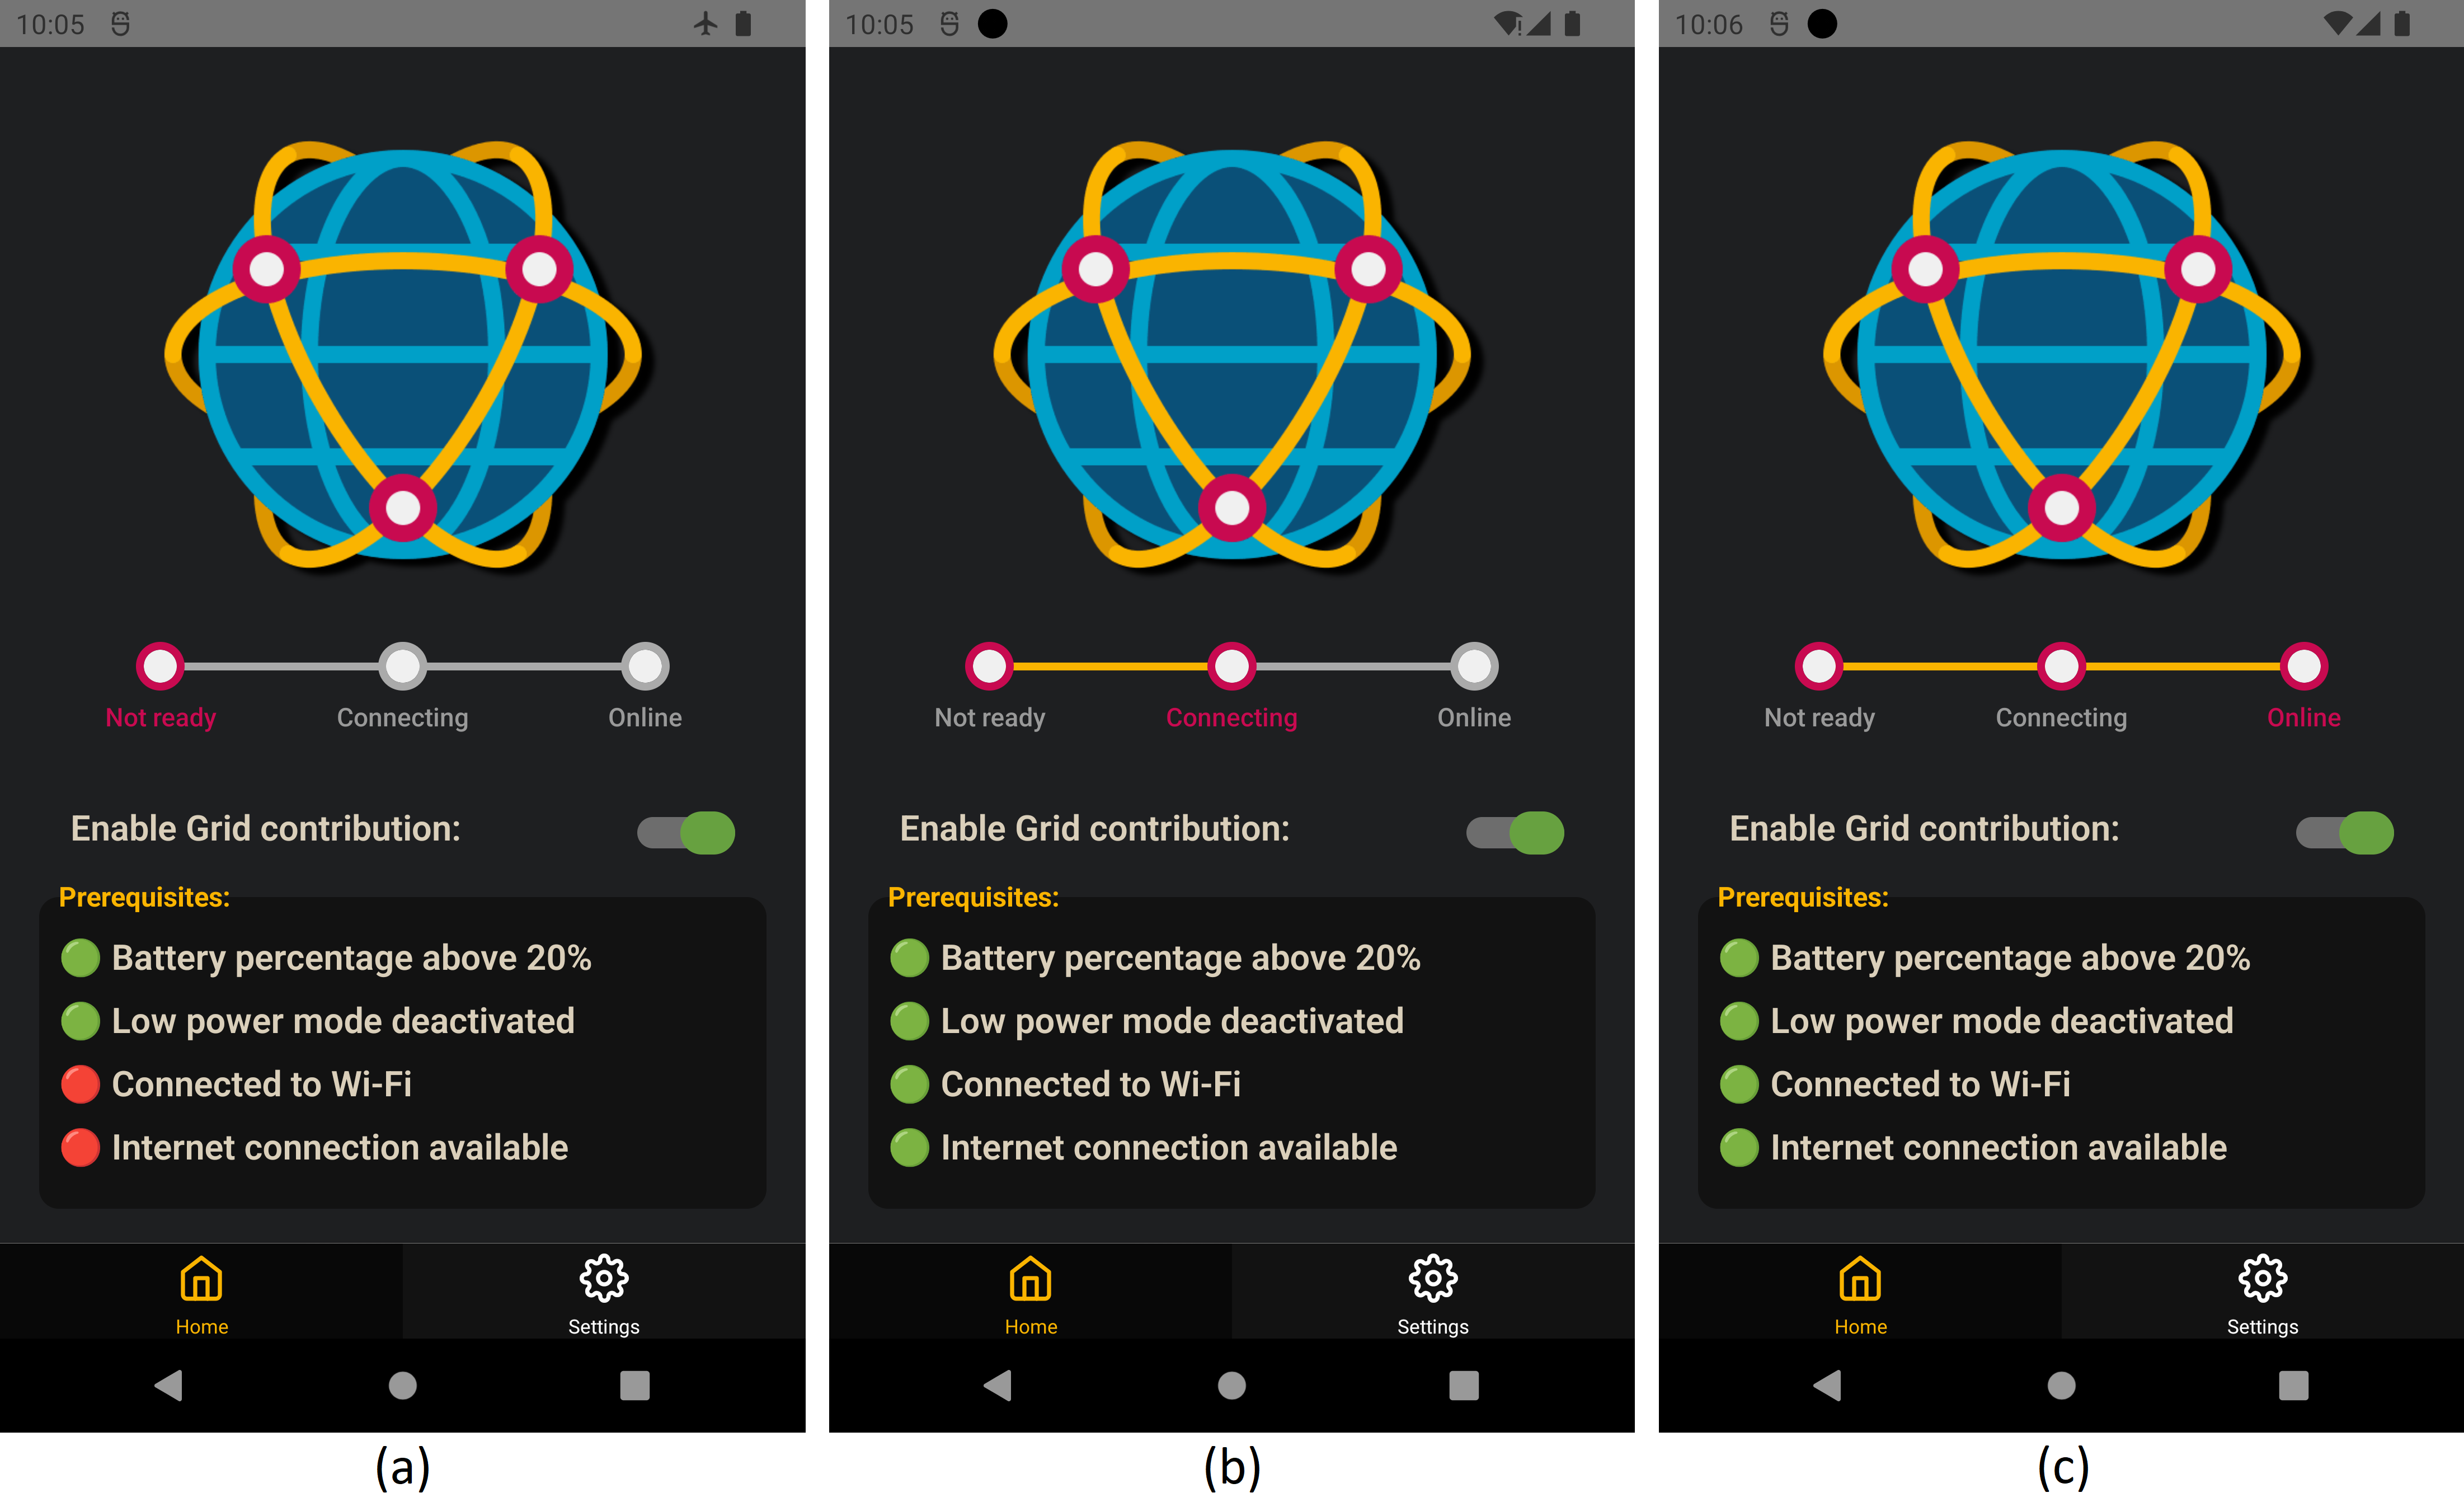
\includegraphics[width=\linewidth]{document/chapters/chapter_7/images/interconnected_mobile_connection.png}
    \caption{Interconnected Mobile Client - Status}
    \label{fig:interconnected_mobile_connection}
\end{figure}

\vspace{5mm}

Despite being a background process, the user can check the application's status through the GUI's indicators: after the activation of the background process, the application remains in the "Not ready" state until all the Prerequisites are met (becoming green); after that, there is a transition to the "Connecting" state (\textit{figure \ref{fig:interconnected_mobile_connection}(b)}) and, once the Grid Connection is established, the "Online" state is reached (\textit{figure \ref{fig:interconnected_mobile_connection}(c)}).

When a contribution to a Grid Service is currently being performed, the user is notified by a notification that, once the contribution is over, is then updated showing that the process is complete (\textit{figure \ref{fig:notification_completed}}).

\begin{figure}[!ht]
    \centering
    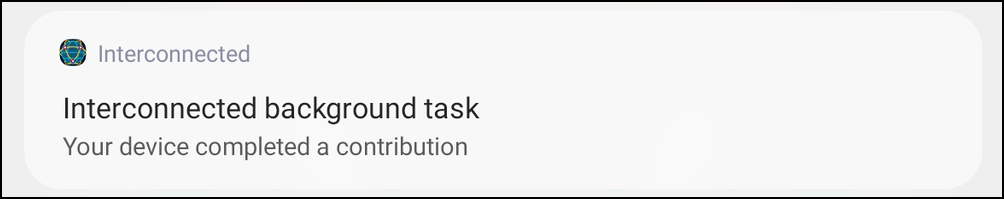
\includegraphics[scale=0.35]{document/chapters/chapter_7/images/notification_completed.png}
    \caption{Interconnected Mobile Client - Grid contribution completed notification}
    \label{fig:notification_completed}
\end{figure}

\subsection{Interconnected Desktop Client}
The Desktop incarnation of the Contributing Endpoint takes the name of "Interconnected Desktop Client"; like the Mobile counterpart, it is developed using the Typescript language and by relying on the Interconnected Node module dependency. For this prototype version no GUI was developed and, then, a simple Docker image (which can run on any computer) is provided.

\begin{figure}[!ht]
    \centering
    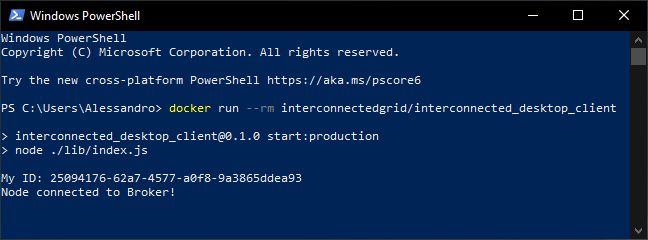
\includegraphics[scale=0.8]{document/chapters/chapter_7/images/interconnected_desktop.png}
    \caption{Interconnected Desktop Client - Docker image run on a container}
    \label{fig:interconnected_desktop}
\end{figure}

In the  as the Interconnected Mobile Client, this prototype's Node ID is generated by using a simple UUID v4 (which can be seen in \textit{figure \ref{fig:interconnected_desktop}}).

\subsection{Invoking Endpoint Prototype}
The last entity that composes this simplified architecture is the Invoking Endpoint Prototype; unlike its counterpart in the complete architecture, which envision it as a dependency (much like the Interconnected Node) which can be used by a Customer Custom application, this prototype version is a standalone program that can interact with the Grid launching a MapReduce computation; more details on the subject will be discussed in \textit{section \ref{real_world_experiments}}.

This entity is developed, like the others, relaying on the Node.js framework but, instead, by using plain JavaScript and not the Typescript superset. In order to be able to communicate with the Broker Service and the Interconnected Nodes, it also utilizes the Socket.io module and the WebRTC module, respectively.